% !Mode:: "TeX:UTF-8" 

\BiChapter{参考文献格式}{Format of References}

参考文献格式应符合国家标准 GB/T-7714-2005《文后参考文献著录规则》。中国国家标准化管理委员会于 2015 年 5 月 15 日发布了新的标准 GB/T 7714-2015《信息与文献参考文献著录规则》。因为二者的差别非常小,所以采用了新的标准。标准的 BiBTeX 格式网上资源非常多,本模板使用了李泽平开发的版本,该版本提供了多种参考文献的排序规则。学校博士论文规范指定了两种排序方法:一是按照文献的引用顺序进行排序,二是按照作者姓氏加出版年份进行排序。本模板采用第一种排序规则,第二种排序规则的使用方法请参考文献\cite{Lee2016}。



虽然本模板不讲解 \LaTeX{} 的详细使用方法,但是为了方便大家使用本模板撰写论文,本章对论文写作中经常用到的{\hei 图、表、公式}等内容的排版方法做一个简单介绍。

%=========================================================================================
\BiSection{图}{Figures}
\BiSubsection{单幅图}{Single Figure}

图 \ref{fig_ch2_echoes} 是用 TeXLive 自带的宏包 Tikz 绘制而成,Visio 画不出这么好看的图。
\begin{figure}[!ht]
	\centering
	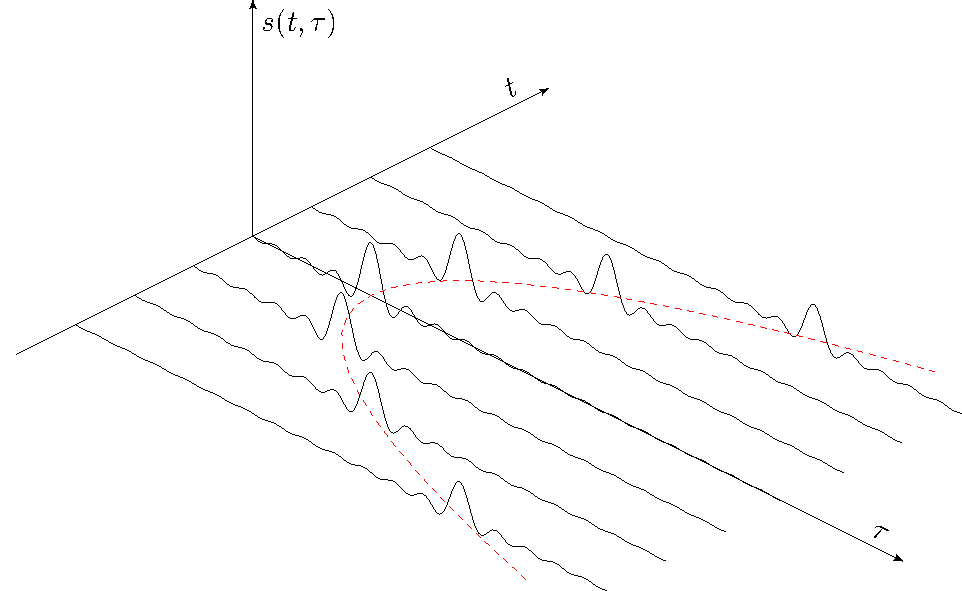
\includegraphics[width=\textwidth]{echoes}
	\caption{雷达回波信号 ({\color{red}注意}:图注是五号字)。} \label{fig_ch2_echoes}
\end{figure}

%-----------------------------------------------------------------------------------------
\BiSubsection{多幅图}{Multiple Figures}

如果一幅图中包含多幅子图,每一幅子图都要有图注,并且子图用 (a)、(b)、(c) 等方式编号,如图 \ref{fig_ch2_badge} 所示。
\begin{figure}[!ht]
	\centering
	\subfigure[灰色的交大校徽]{
\includegraphics[width=0.45\textwidth]{xjtu_gray}} \hfill
	\subfigure[蓝色的交大校徽]{
\includegraphics[width=0.45\textwidth]{xjtu_blue}}
	\caption{交大校徽 \label{fig_ch2_badge}}
\end{figure}

%=========================================================================================
\BiSection{表}{Tables} 

表格要求采用三线表,与文字齐宽,顶线与底线线粗是 $1\frac12$ 磅,中线线粗是 1 磅,如表 \ref{tab_ch2} 所示\footnote{{\color{red}注意}:图表中的变量与单位通过斜线 $/$ 隔开。}。
\begin{table}[!ht]
	\renewcommand{\arraystretch}{1.2}
	\centering\wuhao
	\caption{表题也是五号字} \label{tab_ch2} \vspace{2mm}
	\begin{tabularx}{\textwidth}{*{4}Y}
	\toprule[1.5pt]
		Interference & DOA / degree & Bandwidth / MHz & INR / dB \\
	\midrule[1pt]
		1 & $-30$ & 20 & 60 \\
		2 & 20 & 10 & 50 \\
		3 & 40 & 5 & 40 \\
	\bottomrule[1.5pt]
	\end{tabularx}
\end{table}

%=========================================================================================
\BiSection{公式}{Equations}
\BiSubsection{单个公式}{Equations}

\LaTeX{} 最强大的地方在于对数学公式的编辑,不仅美观,而且高效。单个公式的编号如式 (\ref{equ_ch2_pdf}) 所示,该式是正态分布的概率密度函数\citeup{Manolakis2005},
\begin{equation} \label{equ_ch2_pdf}
	f_Z(z) = \frac{1}{\pi\sigma^2} \exp\left(-\frac{|z-\mu|^2}{\sigma^2}\right)
\end{equation}
式中:$\mu$ 是 Gauss 随机变量 $Z$ 的均值;$\sigma^2$ 是 $Z$ 的方差。

%-----------------------------------------------------------------------------------------
\BiSubsection{多个公式}{Subequations}

多个公式作为一个整体可以进行二级编号,如式 (\ref{equ_ch2_fourier}) 所示,该式是连续时间 Fourier 变换的正反变换公式\citeup{Vetterli2014},
\begin{subequations} \label{equ_ch2_fourier}
	\begin{align}
		X(f) &= \int_{-\infty}^{\infty}x(t)e^{-j2\pi f t}\dif t \\
		x(t) &= \int_{-\infty}^{\infty}X(f)e^{j2\pi f t}\dif f
	\end{align}
\end{subequations}
式中:$x(t)$ 是信号的时域波形;$X(f)$ 是 $x(t)$ 的 Fourier 变换。

如果公式中包含推导步骤,可以只对最终的公式进行编号,例如:
\begin{align}
	\mbf{w}_{\mathrm{smi}} &= \alpha \left[\frac{1}{\sigma_n^2}\mbf{v}(\theta_0) - \frac{1}{\sigma_n^2}\mbf{v}(\theta_0) + \sum_{i=1}^{N} \frac{\mbf{u}_i^H\mbf{v}(\theta_0)}{\lambda_i} \mbf{u}_i\right] \nonumber \\
	&= \frac{\alpha}{\sigma_n^2} \left[\mbf{v}(\theta_0) - \sum_{i=1}^{N}\mbf{u}_i^H\mbf{v}(\theta_0)\mbf{u}_i +  \sum_{i=1}^{N}\frac{\sigma_n^2\mbf{u}_i^H\mbf{v}(\theta_0)}{\lambda_i} \mbf{u}_i \right] \nonumber \\
	&= \frac{\alpha}{\sigma_n^2} \left[\mbf{v}(\theta_0) - \sum_{i=1}^{N} \frac{\lambda_i-\sigma_n^2}{\lambda_i} \mbf{u}_i^H\mbf{v}(\theta_0)\mbf{u}_i \right]
\end{align}